\section{RQ8: When Does Recovery Repay Its Information Cost?}
\label{sec:recovery}

Search savings repay recovery only over a sufficiently long recurring workload. We express the accounting in native distance evaluations,
\begin{equation}
 C_\pi(N)=C_{{\rm acquire},\pi}+N\bar c_\pi,\qquad
 N_{\rm BE}=\frac{\Delta C_{\rm acquire}}{\bar c_{\rm end}-\bar c_\pi}.\label{eq:breakeven}
\end{equation}
If incremental acquisition is positive but serving saving is not, no finite break-even exists. Graph rebuilding is common to both policies on the same target. Control adds no distance calls but is not assigned zero elapsed time.

\paragraph{Two explicit acquisition scenarios.}
With \emph{cached history}, old query profiles and their truth are sunk costs. We charge the complete target-selection grid, the selected candidate's certification searches, additional endpoint-certification searches where the actions differ, and exact target truth for the 1,000 selection/certification queries. Truth is modeled as one scan of 100,000 vectors per query. With \emph{cold complete history}, we also charge sequential old-build profiling for all three roles on all nine contributing histories and exact old-snapshot truth for all 2,000 query IDs. That truth is reusable across old builds of the same collection and is counted once, not nine times. These are workload-acquisition scenarios, not newly measured elapsed-time costs.

We conservatively charge all endpoint certification to recovery, although the reference may also need some of this work. We price the evaluated decision rule without charging repeated calls for the same action and query twice. The earlier partial calculation included old profiling only for evaluation IDs and omitted old truth and extra endpoint certification. Completing these items materially changes the economic conclusion.

\begin{table}[t]
\caption{Joint-error recovery: break-even query executions in thousands [95\% target-build interval], conditional on the finite acquisition workload. The ratio of mean overhead to mean saving is not a per-build guarantee. ``No saving'' counts nonamortizing targets.}
\label{tab:economics}
\small\begin{tabular*}{\linewidth}{@{\extracolsep{\fill}}llrr@{}}\toprule
Dataset & History & Break-even, $10^3$ & No saving\\\midrule
\CostRows
\bottomrule\end{tabular*}
\end{table}

For joint-error replay, cold-history break-even is approximately 396,000 executions on SIFT and 457,000 on Arxiv, versus 129,000 and 148,000 with cached history (Table~\ref{tab:economics}). Four Arxiv targets fall back and never repay a positive recovery overhead through serving savings. The original procedure has lower cold-history break-even on Arxiv, approximately 305,000, but different certification composition. It is therefore insufficient to attach the original economics to the stricter decision rule.

At $N=10^6$, the cold-history joint-error model yields mean net savings of about 490 million NDC on SIFT and 389 million on Arxiv. Their target-build intervals are [488, 491] million and [31, 747] million, respectively. At $10^5$, both cold-history means are negative. Figure~\ref{fig:cost} shows how the crossover depends on what information already exists.

\paragraph{Target-certified fresh-query policy.}
The post-seal replication has a different ledger. Per dataset, the same 500 certification queries are run on every target and reused across its 23 source histories. For each target, exact truth costs $500\times100{,}000$ distances; measured candidate and endpoint searches are added with identical actions deduplicated. Pairwise accounting charges this target audit to every directed source--target unit, whereas shared-target accounting charges it once and reuses it over the 23 registered sources (Table~\ref{tab:target-stage-cost}). On evaluation, mean candidate/endpoint work is 9,169.58/9,997.70 NDC on SIFT and 8,234.58/11,611.52 on Arxiv, yielding the 8.283\% and 29.083\% reductions in Table~\ref{tab:target-certified}. For example, SIFT pairwise acquisition sums to 30.588 billion NDC and serving saving to 457,122.72 NDC per portfolio execution, giving $30.588\text{B}/457{,}122.72=66{,}914$ executions. Shared-target acquisition is 1.380 billion NDC over the same serving saving, giving 3,019 executions. The pairwise/shared acquisition ratio is 22.17 rather than 23 because the shared audit evaluates the union of distinct candidate and endpoint actions for a target, whereas each pairwise audit evaluates only the actions required by that direction. The corresponding Arxiv thresholds are 17,018 and 755. Because clipping gives zero saving in 460/552 and 230/552 directions, the pairwise ratios are portfolio thresholds, not per-direction guarantees.

\begin{table*}[!t]
\caption{Target-stage NDC ledger for the target-certified Faiss candidate. Break-even is a ratio of summed acquisition cost and serving saving [95\% target-build bootstrap interval]. ``No saving'' counts units with zero serving reduction; the final column is the first registered horizon with positive aggregate net NDC.}
\label{tab:target-stage-cost}
\small\begin{tabular*}{\textwidth}{@{\extracolsep{\fill}}llrrrr@{}}\toprule
Dataset & Accounting & Units & Break-even [95\% CI] & No saving & First positive $N$\\\midrule
\TargetStageCostRows
\bottomrule\end{tabular*}
\end{table*}

At $N=10^6$ per direction, mean shared-target net saving per target (aggregated over its 23 source directions) is 18.99 billion NDC on SIFT and 77.61 billion on Arxiv; both target-build interval lower bounds, LOTO minima, and delete-largest-target checks remain positive. This closes the \emph{target-stage} NDC ledger. It does not close complete cold lifecycle economics: historical source-policy acquisition has no compatible per-query NDC record and is not assigned zero. Exact-truth/control wall time is also absent, so search-only timing break-even remains diagnostic rather than an end-to-end latency result.

\begin{figure}[t]
\centering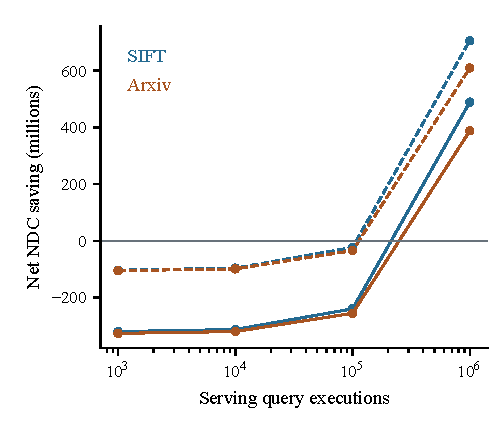
\includegraphics[width=\linewidth]{figures/cost.pdf}
\caption{Joint-error recovery, modeled net distance savings per target versus serving horizon. Solid: cold complete history; dashed: cached history. Dots mark reported horizons; lines depict the stated affine cost model, not additional measurements. Endpoint-fallback targets remain in the average.}
\label{fig:cost}
\Description{Net savings are negative for short horizons and positive at one million executions. Cold-history accounting crosses zero later than cached-history accounting.}
\end{figure}

This calculation assumes repeated executions over the profiled workload. A cache miss requires new information or a declared endpoint action; an unbounded stream of new query identities can invalidate the amortization. Acquisition of historical graphs themselves is not reconstructed here: cold history means acquiring profiles on retained graphs, not rebuilding the entire archive. Memory traffic, storage, energy, and control time require separate prices. The result is a conditional distance-work benefit, not an end-to-end latency or monetary claim.
